\chapter{Vyhodnotenie navrhovaného riešenia}\label{ch:vyhodnotenie-navrhovaneho-riesenia}

Primárnym výsledkom nášho navrhovaného riešenia bolo zabezpečenie prístupu na vzdialené zariadenie za účelom zasielania príkazov
spolu s dôvernými údajmi.
Samotný prístup na koncové zariadenia musí spĺňať bezpečnostné požiadavky vo všetkých fázach implementovaného prípadu
použitia.
Ďalším dôležitým cieľom bolo zaistenie komunikácie medzi jednotlivými časťami systému a modulárne navrhnúť všetky potrebné
súčasti tak, aby ich bolo možné s pribúdajúcimi kritériami bezpečnosti, alebo použitia jednoducho doimplementovať.

Pri nasadení nášho riešenia v systéme figuruje iba používateľ typu „superuser“, ktorý má všetky systémové práva.
Tento používateľ vie vykonať potrebné akcie, ako napríklad: vytvorenie projektov, definícií koncových zariadení, oprávnenia,
ďalších používateľov a iné entity, ktoré sú nevyhnutné pre správne fungovanie systému.

\section{Vytvorenie používateľa a autentifikácia}\label{sec:vytvorenie-pouzivatela-autentifikacia}

Vytvorenie používateľa s rolou „devops“ je po prihlásení superuserom nasledovné:

\textbf{\large Požiadavka [POST]:}

\begin{lstlisting}[language=json,firstnumber=1]
{
  "email": "devops@praetorian.sk",
  "password": "devops",
  "name": "devops",
  "surname": "devops",
  "role": "devops",
  "is_vpn": false,
  "additional_data": {},
  "language_id": "ee3f8e7a-c9d8-4d96-8dd0-816775b25b7d"
}
\end{lstlisting}

\textbf{\large Odpoveď:}

\begin{lstlisting}[language=json,firstnumber=1]
{
  "response": {
    "id": "dbab895b-5568-45bf-95a3-55d96118836c",
    "username": "devops@praetorian.sk",
    "name": "devops",
    "surname": "devops",
    "email": "devops@praetorian.sk",
    "role": "devops",
    "additional_data": {}
  }
}
\end{lstlisting}

Po úspešnom vytvorení používateľa a po registrovaní jeho zariadenia v systéme, je mu superuserom možné priradiť jeden z
existujúcich projektov v systéme a následne sa za neho prihlásiť:

\textbf{\large Požiadavka [POST]:}

\begin{lstlisting}[language=json,firstnumber=1]
{
  "username": "devops@praetorian.sk",
  "password": "devops"
}
\end{lstlisting}

\textbf{\large Odpoveď:}

\begin{lstlisting}[language=json,firstnumber=1]
{
  "response": {
    "token": "22fcf8a5-7c90-4e3a-a665-7cf842b46283",
    "active_2fa": false
  }
}
\end{lstlisting}

Ako je z odpovede webového api rozhrania vidieť, používateľ nie je overený dvojfaktorovou autentifikáciou.
Táto hodnota sa v odpovedi nachádza z dôvodu informovania, či je potrebné vyžiadanie tohto dodatočného typu autentifikácie.

Pre vyžiadanie dvojfaktorovej autentifikácie je potrebné si danú službu aktivovať nasledovným spôsobom:

\textbf{\large Požiadavka [GET]:}

\inlinecode{\{\{ api\_url \}\}/v1/users/\{\{ user\_id \}\}/2fa/}

\newpage
\textbf{\large Odpoveď:}

\begin{lstlisting}[language=json,firstnumber=1]
{
  "response": {
    "qr_code": "otpauth://totp/Praetorian%20API:devops%40praetorian.sk?secret=J4UZONZ36IQGLZAM&issuer=Praetorian%20API"
  }
}
\end{lstlisting}

Reťazec v odpovedi slúži na vytvorenie qr kódu, ktorý bude zobrazený v grafickom užívateľskom rozhraní, pričom používateľ
je o aktivácii dvojfaktorovej autentifikácie taktiež informovaný pomocou zaslaného systémového emailu, ktorého obsah
je na obrázku ~\ref{fig:obr_13}. Keďže OTP je citlivý údaj, komunikácia medzi api serverom a frontend api musí prebiehať
za pomoci šifrovanej komunikácie HTTPS.
Bezpečnosť je možné dodatočne rozšíriť šifrovaním posielaného response body, ktorý by bol dešifrovaný na strane frontend api.
Tým by sa minimalizovalo riziko odchytenia tohto citlivého údaju treťou stranou odpočúvajúcu komunikáciu.

\begin{figure}[H]
\begin{center}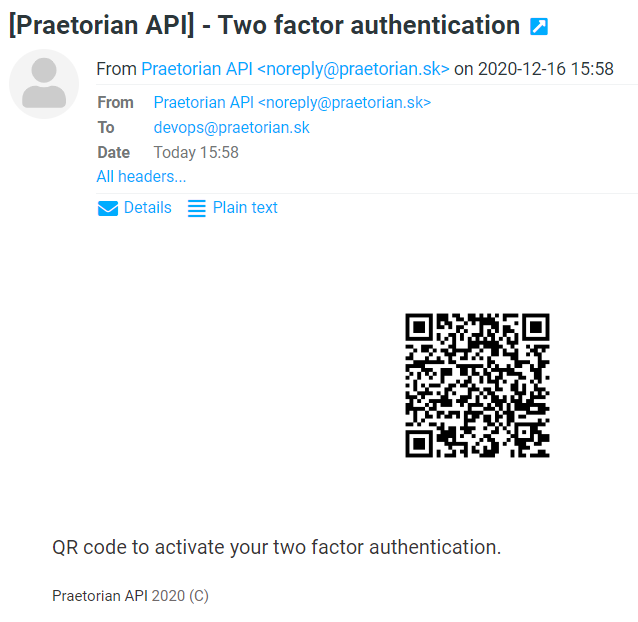
\includegraphics[width=\textwidth,height=9cm,keepaspectratio=true]{assets/2fa_email.png}\end{center}
\caption[Obsah emailu informujúcom o aktivácii dvojfaktorovej autentifikácie]{Obsah emailu informujúcom o aktivácii dvojfaktorovej autentifikácie}\label{fig:obr_14}
\end{figure}

Naskenovaním daného qr kódu, napríklad v aplikácii „Authenticator“, sa vytvorí nový účet, ktorému je priradený práve jeden OTP
s veľmi krátkou životnosťou.
Po uplynutí životnosti sa OTP automaticky pregeneruje.
Vytvorený účet v aplikácii Authenticator so zobrazeným OTP je znázornený na obrázku~\ref{fig:obr_15}.

\begin{figure}[H]
\begin{center}
\includegraphics[width=\textwidth,height=9cm,keepaspectratio=true]{assets/authenticator.png}\end{center}
\caption[Zobrazenie aktivovaného účtu s OTP v aplikácii Authenticator]{Zobrazenie aktivovaného účtu s OTP v aplikácii Authenticator}\label{fig:obr_15}
\end{figure}

\section{Interaktívny SSH session}\label{sec:interaktivny-ssh-session}

Ďalšou z možností nami vytvoreného používateľa je pripojenie sa na vzdialené zariadenie pomocou ssh proxy servera, pričom na
pripojenie je použité interaktívne prostredie.
Celý proces pripojenia používateľa ku koncovému zariadeniu je zobrazený na obrázku~\ref{fig:obr_16}.

\begin{figure}[H]
\begin{center}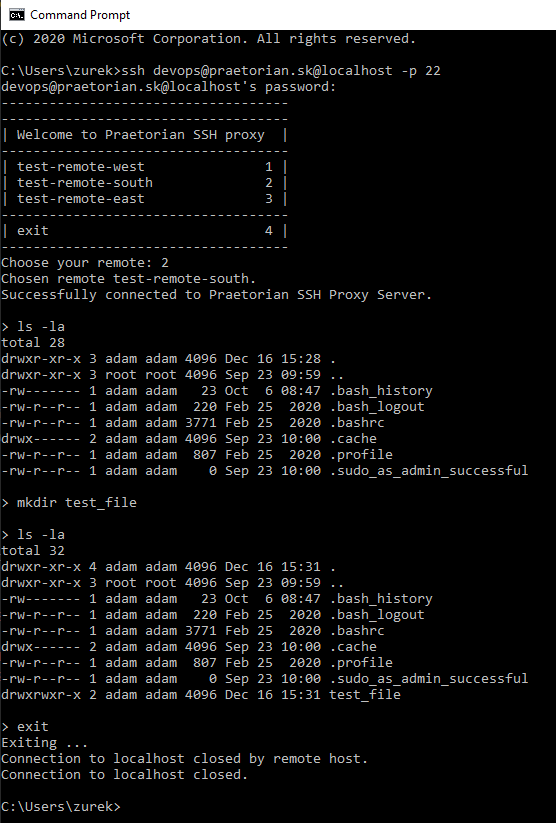
\includegraphics[width=\textwidth,height=20cm,keepaspectratio=true]{assets/interactive_session.png}\end{center}
\caption[Proces pripojenia cez interaktívne prostredie]{Proces pripojenia cez interaktívne prostredie}\label{fig:obr_16}
\end{figure}

Keďže si používateľ nezvolil koncové zariadenie, ssh proxy server mu ponúkol zoznam dostupných zariadení, ku ktorým má daný používateľ
právo. Používateľ po úspešnom pripojení na zvolené koncové zariadenie cez interaktívne prostredie vytvoril na koncovom zariadení
priečinok s názvom „test\_file\_1“. Následne si prezrel históriu bash a úspešne sa z danej relácie odpojil.
Interaktívnym spôsobom sa používateľ vie pripojiť na koncové zariadenie aj priamo bez nutnosti výberu, čo je zobrazené na
obrázku~\ref{fig:obr_17}.

\begin{figure}[H]
\begin{center}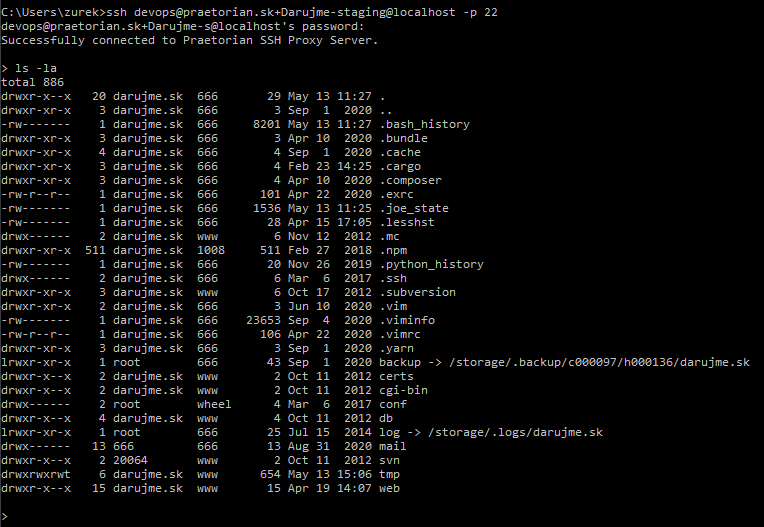
\includegraphics[width=\textwidth,height=10cm,keepaspectratio=true]{assets/direct_interactive_session.png}\end{center}
\caption[Priame pripojenie cez interaktívne prostredie]{Priame pripojenie cez interaktívne prostredie}\label{fig:obr_17}
\end{figure}

\section{Neinteraktívny SSH session}\label{sec:neinteraktivny-ssh-session}

Neinteraktívny mód riešenia môže byť demonštrovaný a otestovaný vytvorením skriptu, ktorý bude mazať súbor „test\_file\_1“.
Skript bude pozostávať z troch príkazov:

\begin{enumerate}
  \item \inlinecode{ls -la}
  \item \inlinecode{rmdir test\_file\_1}
  \item \inlinecode{ls -la}
\end{enumerate}

Neinteraktívny mód vyžaduje vytvorenie dočasného používateľa, ktorého úlohou bude daný skript jednorázovo vykonať, pričom bude po
dokončení úlohy dočasný požívateľ vymazaný.
Pre vytvorenie dočasného používateľa je potrebné sa prihlásiť za permanentného používateľa do webového api rozhrania a
vytvoriť nasledovnú požiadavku:

\textbf{\large Požiadavka [POST]:}

\begin{lstlisting}[language=json,firstnumber=1]
{
  "project_id": "408c57f3-6ea4-42dc-beb3-a0051b97182f",
  "remote_id": "f2228baf-d999-4d7a-9780-b8f2be97956f"
}
\end{lstlisting}

\textbf{\large Odpoveď:}

\begin{lstlisting}[language=json,firstnumber=1]
{
  "response": {
    "username": "jPTgEYC@praetorian.sk",
    "password": "AnVV6kLPA9"
  }
}
\end{lstlisting}

Používateľovi taktiež v prípade zabudnutia prístupových údajov k dočasnému používateľovi dôjde notifikácia s potrebnými
informáciami, ktorej obsah je zobrazený na obrázku~\ref{fig:obr_18}.

\begin{figure}[H]
\begin{center}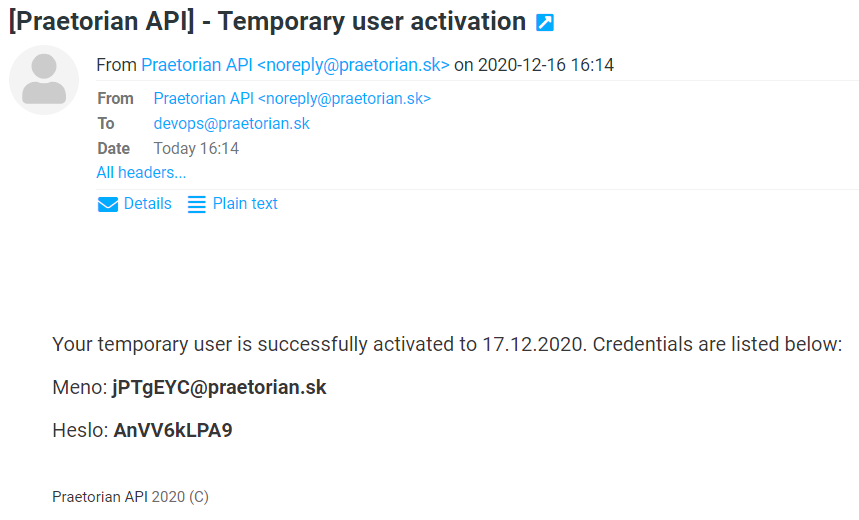
\includegraphics[width=\textwidth,height=10cm,keepaspectratio=true]{assets/temporary_credentials.png}\end{center}
\caption[Obsah emailu informujúcom o prístupových údajoch dočasného používateľa]{Obsah emailu informujúcom o prístupových údajoch dočasného používateľa}\label{fig:obr_18}
\end{figure}

Po úspešnom vytvorení skriptu a dočasného používateľa je možné sa pripojiť na koncové zariadenie cez neinteraktívne prostredie,
ktorého vykonanie je na obrázku~\ref{fig:obr_19}.

\begin{figure}[H]
\begin{center}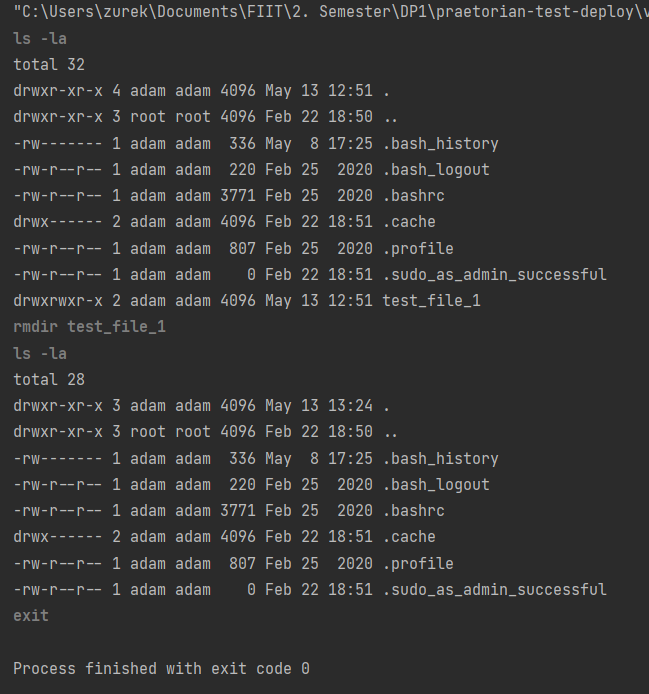
\includegraphics[width=\textwidth,height=12cm,keepaspectratio=true]{assets/non_interactive_session.png}\end{center}
\caption[Proces pripojenia cez neinteraktívne prostredie]{Proces pripojenia cez neinteraktívne prostredie}\label{fig:obr_19}
\end{figure}

Po úspešnom dokončení vykonávania príkazov na dané koncové zariadenie, bolo nasledovne ukončené spojenie a dočasný používateľ
bol vymazaný.

\subsection{Nasadenie finálneho produktu}\label{subsec:nasadenie-finalneho-produktu}

Daný príklad ukazoval hlavné rozdiely medzi interaktívnym a neinteraktívnym pripojením. No využitie neinteraktívneho pripojenia
vie byť rozšírené o manipuláciu s citlivými údajmi a rozsiahly proces nasadenia finálneho produktu používaného v praxi.
V nasledovnom príklade sa jedná o portál \emph{https://darujme.sk/}, ktorý je naše riešenie schopné nasadiť na koncové zariadenie
s úplnou anonymizáciou prístupových údajov. Na nasledujúcom obrázku vidíme časť skriptu, ktorý sa na nasadenie použije~\ref{fig:obr_20}.

\begin{figure}[H]
\begin{center}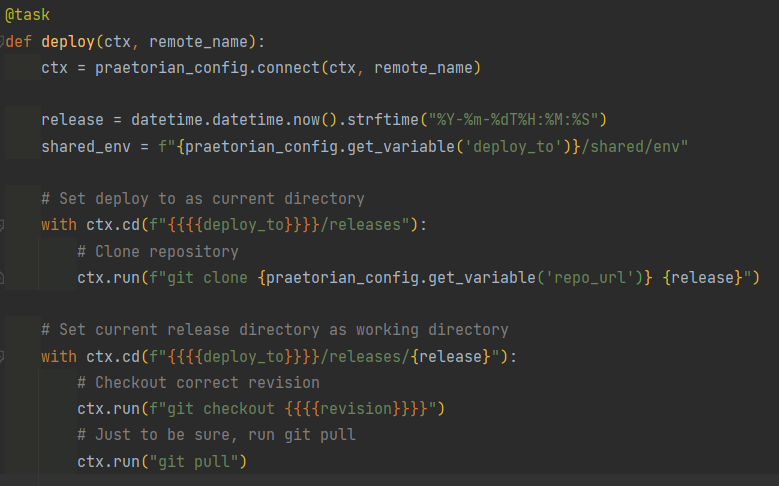
\includegraphics[width=\textwidth,height=12cm,keepaspectratio=true]{assets/deploy_script.png}\end{center}
\caption[Ukážka skriptu nasadzujúceho finálny produkt]{Ukážka skriptu nasadzujúceho finálny produkt}\label{fig:obr_20}
\end{figure}

V skripte môžme vidieť spomínané pripojenie na ssh proxy server cez objekt typu \inlinecode{PraetorianConfig}, kde dopyt
po menej dôverných údajoch sa vykonáva cez metódu \inlinecode{get\_value}, ktorá vráti aktuálnu hodnotu informácie.
Hodnoty, ktoré sú dôverné a používateľ k ním nemá prístup sa volajú svojim názvom ohraničeným kučeravými zátvorkami.
Tento príkaz je následne po prijatí ssh proxy serverom analyzovaný, pričom všetky názvy informácií nahradí hodnotami a následne
odošle na koncové zariadenie. Časť priebehu celého procesu nasadenia z pohľadu používateľovho zariadenia môžme vidieť na
obrázku~\ref{fig:obr_21}.

\begin{figure}[H]
\begin{center}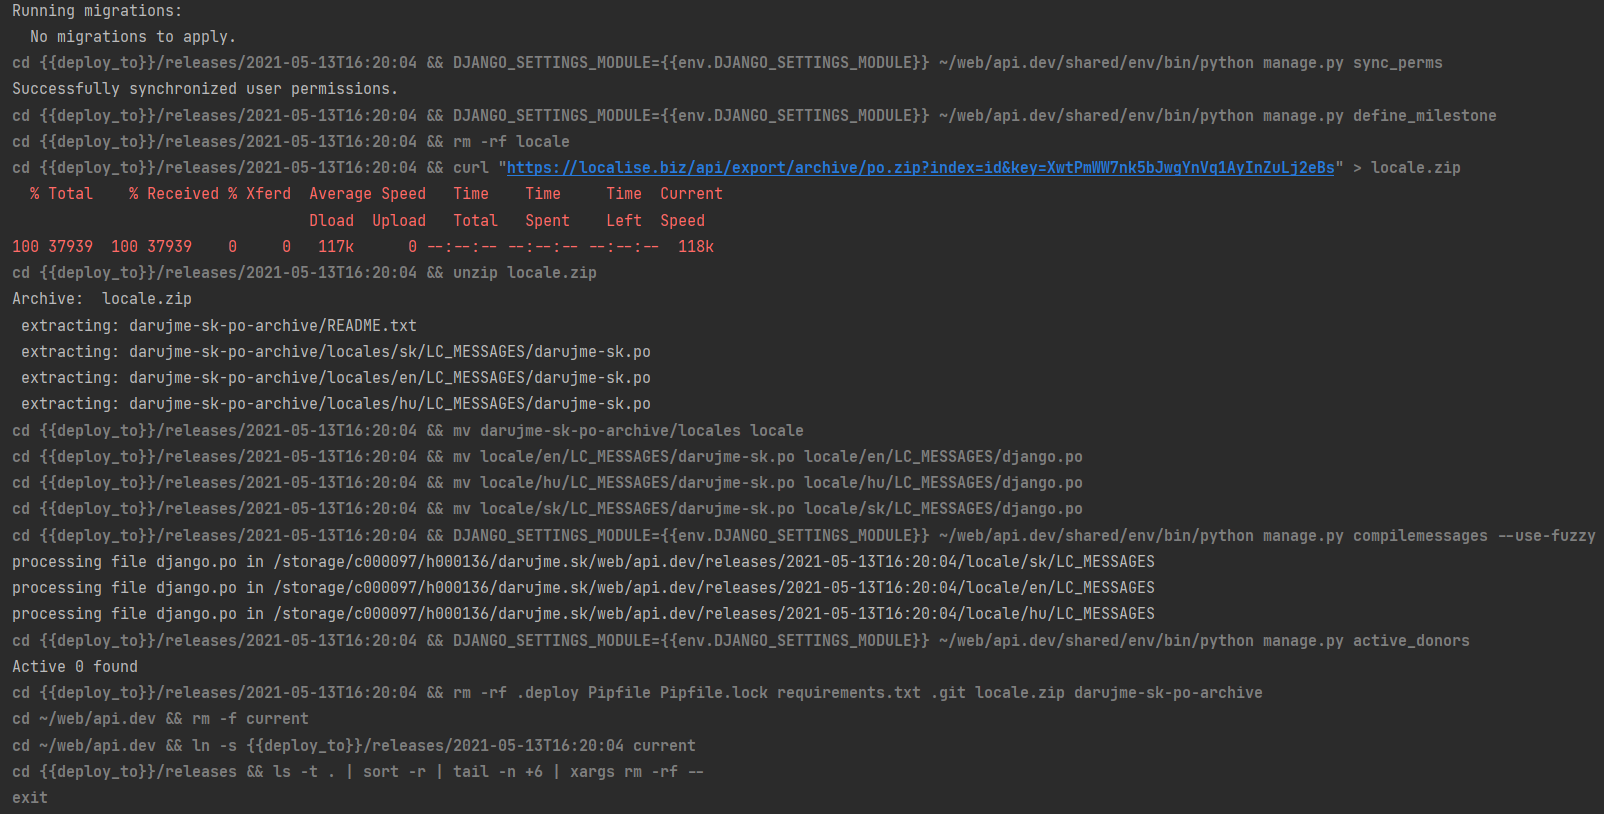
\includegraphics[width=\textwidth,height=12cm,keepaspectratio=true]{assets/log_deploy_user.png}\end{center}
\caption[Priebeh procesu nasadenia zo strany používateľa]{Priebeh procesu nasadenia zo strany používateľa}\label{fig:obr_21}
\end{figure}

Z obrázka~\ref{fig:obr_21} vidíme, že citlivé informácie nie sú používateľovi prístupné žiadnou formou a zobrazované sú
iba svojim názvom aj vo výstupe z logovacieho procesu. Na druhej strane ssh proxy server má taktiež svoj logovací systém, pričom mu môže byť
nastavená rôzna škála miery logovania. Na obrázku~\ref{fig:obr_22} je zobrazený proces analýzy a nahradenia názvov dôverných
informácií skutočnými hodnotami, ktoré sú následne zaslané vo forme príkazu na koncové zariadenie.

\begin{figure}[H]
\begin{center}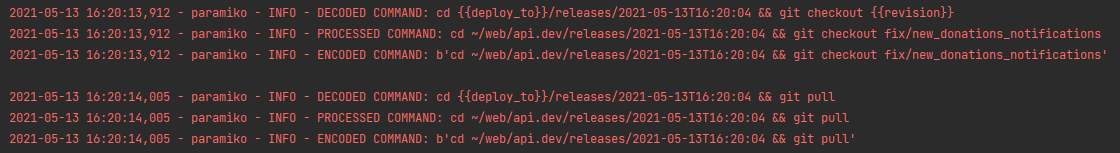
\includegraphics[width=\textwidth,height=12cm,keepaspectratio=true]{assets/log_deploy_proxy}\end{center}
\caption[Priebeh procesu nasadenia zo strany proxy servera]{Priebeh procesu nasadenia zo strany proxy servera}\label{fig:obr_22}
\end{figure}

Vytvorenie dočasného používateľa sa v tomto prípade vykonáva cez rozšírenie knižnice fabric automaticky. Tým pádom nie je nutné
vykonávať manuálny medzi krok.

\section{Zhodnotenie}\label{sec:zhodnotenie}

Systém obsahuje značné množstvo elementárnych funkcionalít ako napríklad: Manažment používateľov, projektov, skupín,
monitorovanie všetkých systémových akcií, kontrola povolených zariadení a mnoho ďalších.
Tieto operácie neboli primárnou oblasťou nášho záujmu a preto sme sa pri testovaní a vyhodnocovaní riešenia zamerali na
najdôležitejšie a kľúčové prípady použitia, ktoré spadali do oblasti nášho výskumu.

Výsledky testovaných scenárov boli očakávané, a teda potvrdili hlavý účel našej práce, čo je správa citlivých a prístupových údajov
spolu s možnosťou bezpečnej a anonymizovanej komunikácie na koncové zariadenia zákazníkov v praxi, bez akejkoľvek nutnosti
používateľa operovať nad citlivými a dôvernými údajmi.

Testovanie najskôr prebehlo v lokálnom prostredí, kde boli všetky komponenty riešenia na jednom zariadení. Neskôr bolo testovanie
uskutočňované na predpripravených testovacích prostrediach priamo určených ako sandbox.
Poslednou iteráciou a výsledným testom bola správa, komunikácia a nasadzovanie produktov v praxi na koncové zariadenia zákazníkov
v softvérovej spoločnosti Backbone s.r.o., pričom jednotlivé komponenty riešenia boli nasadené na rôznych zariadeniach a komunikácia
prebiehala medzi rôznymi druhmi sietí vrátane lokálnej firemnej siete a pripojenia cez vpn.

Pri testovaní systému nenastali žiadne závažné problémy a všetky operácie od manažovania a správy entít v systéme, cez
monitorovanie, až po nasadzovanie a pripájanie sa na koncové zariadenia prebehli hladko.
